\documentclass{article}

% Packages required to support encoding
\usepackage{ucs}
\usepackage[utf8x]{inputenc}
\usepackage{graphicx} 
% Packages required by code

% Packages always used
\usepackage{listings}
\usepackage{hyperref}
\usepackage{xspace}
\usepackage[usenames,dvipsnames]{color}
\hypersetup{colorlinks=true,urlcolor=blue}


\usepackage[framed,numbered,autolinebreaks,useliterate] {mcode}


\usepackage{geometry}
\geometry{letterpaper,textwidth=350pt,textheight=680pt,tmargin=60pt,
            left=72pt,footskip=24pt,headsep=18pt,headheight=14pt}
\usepackage{amsmath}
\usepackage{amssymb}
\usepackage{textcase}
\usepackage{soul}

\newcommand{\mat}[1]{\boldsymbol{#1}}\renewcommand{\vec}[1]{\boldsymbol{\mathrm{#1}}}
\newcommand{\vecalt}[1]{\boldsymbol{#1}}

\newcommand{\conj}[1]{\overline{#1}}

\newcommand{\normof}[1]{\|#1\|}
\newcommand{\onormof}[2]{\|#1\|_{#2}}

\newcommand{\itr}[2]{#1^{(#2)}}
\newcommand{\itn}[1]{^{(#1)}}

\newcommand{\eps}{\varepsilon}
\newcommand{\kron}{\otimes}

\DeclareMathOperator{\diag}{diag}
\DeclareMathOperator{\trace}{trace}
\DeclareMathOperator{\tvec}{vec}

\newcommand{\prob}{\mathbb{P}}
\newcommand{\probof}[1]{\prob\left\{ #1 \right\}}

\newcommand{\pmat}[1]{\begin{pmatrix} #1 \end{pmatrix}}
\newcommand{\bmat}[1]{\begin{bmatrix} #1 \end{bmatrix}}
\newcommand{\spmat}[1]{\left(\begin{smallmatrix} #1 \end{smallmatrix}\right)}
\newcommand{\sbmat}[1]{\left[\begin{smallmatrix} #1 \end{smallmatrix}\right]}

\newcommand{\RR}{\mathbb{R}}
\newcommand{\CC}{\mathbb{C}}

\providecommand{\eye}{\mat{I}}
\providecommand{\mA}{\ensuremath{\mat{A}}}
\providecommand{\mB}{\ensuremath{\mat{B}}}
\providecommand{\mC}{\ensuremath{\mat{C}}}
\providecommand{\mD}{\ensuremath{\mat{D}}}
\providecommand{\mE}{\ensuremath{\mat{E}}}
\providecommand{\mF}{\ensuremath{\mat{F}}}
\providecommand{\mG}{\ensuremath{\mat{G}}}
\providecommand{\mH}{\ensuremath{\mat{H}}}
\providecommand{\mI}{\ensuremath{\mat{I}}}
\providecommand{\mJ}{\ensuremath{\mat{J}}}
\providecommand{\mK}{\ensuremath{\mat{K}}}
\providecommand{\mL}{\ensuremath{\mat{L}}}
\providecommand{\mM}{\ensuremath{\mat{M}}}
\providecommand{\mN}{\ensuremath{\mat{N}}}
\providecommand{\mO}{\ensuremath{\mat{O}}}
\providecommand{\mP}{\ensuremath{\mat{P}}}
\providecommand{\mQ}{\ensuremath{\mat{Q}}}
\providecommand{\mR}{\ensuremath{\mat{R}}}
\providecommand{\mS}{\ensuremath{\mat{S}}}
\providecommand{\mT}{\ensuremath{\mat{T}}}
\providecommand{\mU}{\ensuremath{\mat{U}}}
\providecommand{\mV}{\ensuremath{\mat{V}}}
\providecommand{\mW}{\ensuremath{\mat{W}}}
\providecommand{\mX}{\ensuremath{\mat{X}}}
\providecommand{\mY}{\ensuremath{\mat{Y}}}
\providecommand{\mZ}{\ensuremath{\mat{Z}}}
\providecommand{\mLambda}{\ensuremath{\mat{\Lambda}}}
\providecommand{\mPbar}{\bar{\mP}}

\providecommand{\ones}{\vec{e}}
\providecommand{\va}{\ensuremath{\vec{a}}}
\providecommand{\vb}{\ensuremath{\vec{b}}}
\providecommand{\vc}{\ensuremath{\vec{c}}}
\providecommand{\vd}{\ensuremath{\vec{d}}}
\providecommand{\ve}{\ensuremath{\vec{e}}}
\providecommand{\vf}{\ensuremath{\vec{f}}}
\providecommand{\vg}{\ensuremath{\vec{g}}}
\providecommand{\vh}{\ensuremath{\vec{h}}}
\providecommand{\vi}{\ensuremath{\vec{i}}}
\providecommand{\vj}{\ensuremath{\vec{j}}}
\providecommand{\vk}{\ensuremath{\vec{k}}}
\providecommand{\vl}{\ensuremath{\vec{l}}}
\providecommand{\vm}{\ensuremath{\vec{l}}}
\providecommand{\vn}{\ensuremath{\vec{n}}}
\providecommand{\vo}{\ensuremath{\vec{o}}}
\providecommand{\vp}{\ensuremath{\vec{p}}}
\providecommand{\vq}{\ensuremath{\vec{q}}}
\providecommand{\vr}{\ensuremath{\vec{r}}}
\providecommand{\vs}{\ensuremath{\vec{s}}}
\providecommand{\vt}{\ensuremath{\vec{t}}}
\providecommand{\vu}{\ensuremath{\vec{u}}}
\providecommand{\vv}{\ensuremath{\vec{v}}}
\providecommand{\vw}{\ensuremath{\vec{w}}}
\providecommand{\vx}{\ensuremath{\vec{x}}}
\providecommand{\vy}{\ensuremath{\vec{y}}}
\providecommand{\vz}{\ensuremath{\vec{z}}}
\providecommand{\vpi}{\ensuremath{\vecalt{\pi}}}

\sodef\allcapsspacing{\upshape}{0.15em}{0.65em}{0.6em}%

\makeatletter
\def\maketitle{%
\par
\hrule height 0.75pt\vspace{1ex}
\par\noindent
\begin{minipage}{0.5\textwidth}
\scshape
purdue university $\cdot$ CS 580 \\
Introduction to the Analysis of Algorithms
\end{minipage}
\begin{minipage}{0.5\textwidth}
\raggedleft
\MakeTextUppercase{\allcapsspacing{\@title}}\\[0.2ex]
\textit{\@author}\\[0.2ex]
\textit{\@date}
\end{minipage}
\par\vspace{1ex}
\hrule height 1pt
\vspace{2ex}
\par
}
\makeatother

\author{Jun Cheng}
\title{Lecture Notes}
% auto generate a title
\AtBeginDocument{\maketitle}


\title{Homework}



\begin{document} 



\hypertarget{problem_0_homework_checklist_2}{}
\subsection*{{Problem 1}}
\label{problem_0_homework_checklist_2}

For equation $f(x) = e^{-x}-x=0 $  \newline
$f(0)=1>0$ and $f(1)=e^{-1}-1<0$.  Also function $f(x)$ is continuous monotonic decreasing function.Therefore there must be a root on the interval $(0,1) $ \newline
For the first 4 iterations.  interval [a, b] becomes: \\
\begin{itemize}
\item iter0: [0,		1	 ]\\
\item iter1: [0.5,	1	 ]\\
\item iter2: [0.5,		0.75	 ]\\
\item iter3: [0.5,		0.625]\\
\item iter4: [0.5625,	0.625]\\
\end{itemize}
Therefore $p_3=0.625$ and $(a_4, b_4)=(0.5625, 0.625) $



\hypertarget{problem_0_homework_checklist_2}{}
\subsection*{{Problem 2}}
\label{problem_0_homework_checklist_2}

For equation $f(x) = x_6-3=0 $  \newline
$f(1)=-2<0$ and $f(2)=61>0$.  Also function $f(x)$ is continuous monotonic increasing function.Therefore there must be a root on the interval $(1,2) $ \newline

Output from bisection code: \\
\begin{itemize}
\item iter0 [1,	2] \\
\item iter1 [1,	1.5]   		:actual error $ |1.5-\sqrt[6]{3}|=0.299< 0.5$ \\
\item iter2 [1,	1.25]			:actual error $ |1.25-\sqrt[6]{3}|=0.049< 0.25$ \\
\item iter3 [1.125,	1.25]		:actual error $ |1.125-\sqrt[6]{3}|=0.0759< 0.125$ \\
\item iter4 [1.1875,	1.25]		:actual error $ |1.1875-\sqrt[6]{3}|=0.0134< 0.0625$ \\
\item iter5 [1.1875,	1.21875]	:actual error $ |1.21875-\sqrt[6]{3}|=0.0178< 0..03125$ \\
\end{itemize}
We can see that each approximation satisfies the theoretical error, but the actual error does not steadily decrease. Sometimes it is large and sometimes it is small. \\

\hypertarget{problem_3_homework_checklist_2}{}
\subsection*{{Problem 3}}
\label{problem_0_homework_checklist_2}
For each step the error would become half of the interval. So 
\begin{align} 
error_n = \frac{(b-a)}{2^n}\\
\epsilon > error_n\\
\epsilon >  \frac{(b-a)}{2^n}\\
n>\log_2 \frac{(b-a)}{\epsilon}\\
\end{align}
Therefore $n$ should be the integer bigger than $\log_2 \frac{(b-a)}{\epsilon}$

\hypertarget{problem_4_homework_checklist_2}{}
\subsection*{{Problem 4}}
\label{}
\begin{enumerate}
\item 
See output of attached code.  The result is 1.73205. 
\item 
For the first 5 iterations: \\
 $|p_n-p_{n-1}|, \quad    |p_{n-1}-p|,   \quad  |p_n-p|  $\\
0.277778,  \quad   0.232051,   0.045727\\
0.0444171, \quad	0.045727,  \quad	0.00130986\\
0.00130874, \quad	0.00130986, \quad	1.12184e-06\\
1.12184e-06, \quad	1.12184e-06,\quad 8.24008e-13\\
8.23785e-13, \quad	 8.24008e-13, \quad   2.22045e-16\\
\item 
The ratios of $|p_n-p|/|p_{n-1}-p|^2$: \\
\begin{itemize}
\item 0.849193\\
\item 0.62644\\
\item 0.653856\\
\item 0.65474\\
\end{itemize}
Which is approaches to $|f''(p)/2f'(p)|=0.654701 $
\end{enumerate}


\hypertarget{problem_5_homework_checklist_2}{}
\subsection*{{Problem 5}}
\label{}
The true value is : 2.35134\\
The estimated value is 2.351
 \begin{figure}
 \centering 
 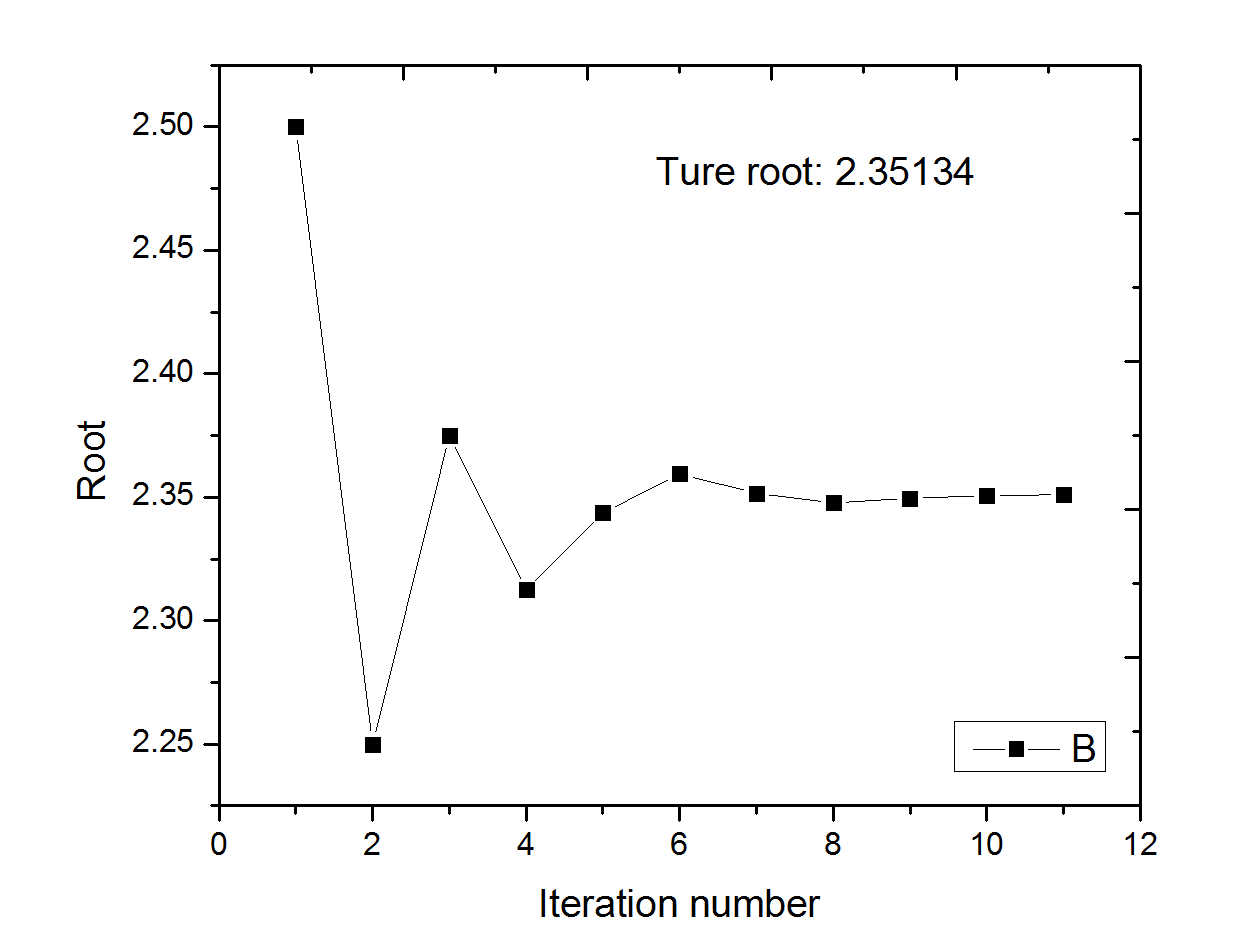
\includegraphics[width=0.5\textwidth]{root}
 \caption{Problem 5. Root vs interation number} 
 \end{figure} 
  \begin{figure}
  \centering 
 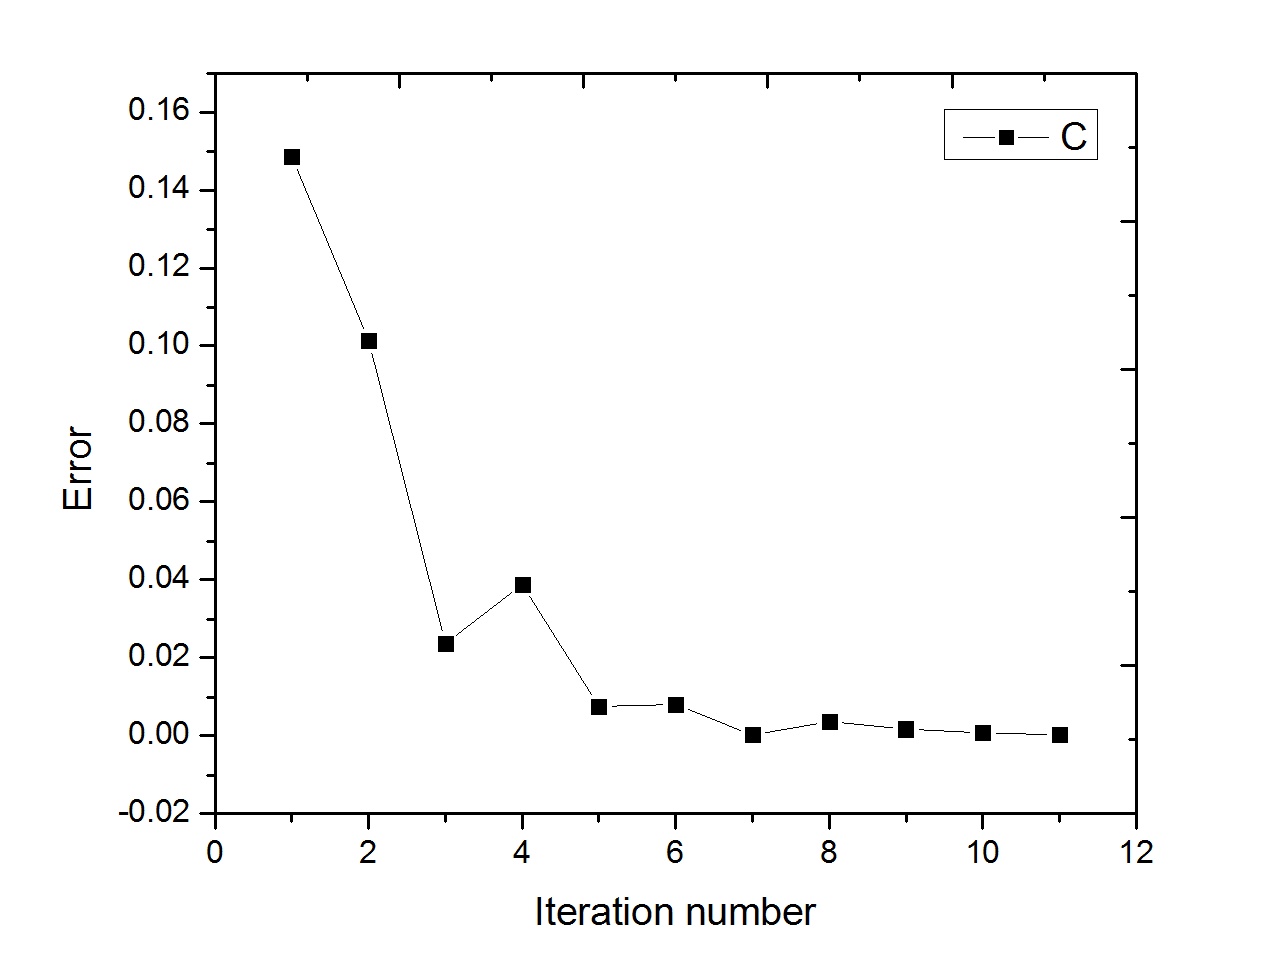
\includegraphics[width=0.5\textwidth]{error}
  \caption{Problem 5. Error vs interation number} 
 \end{figure} 


\hypertarget{problem_6_homework_checklist_2}{}
\subsection*{{Problem 6}}
\label{}
The true value (from Wolfram Alpha)  is : 1.45757030926521\\
The estimated value is 1.45757
 \begin{figure}
 \centering 
 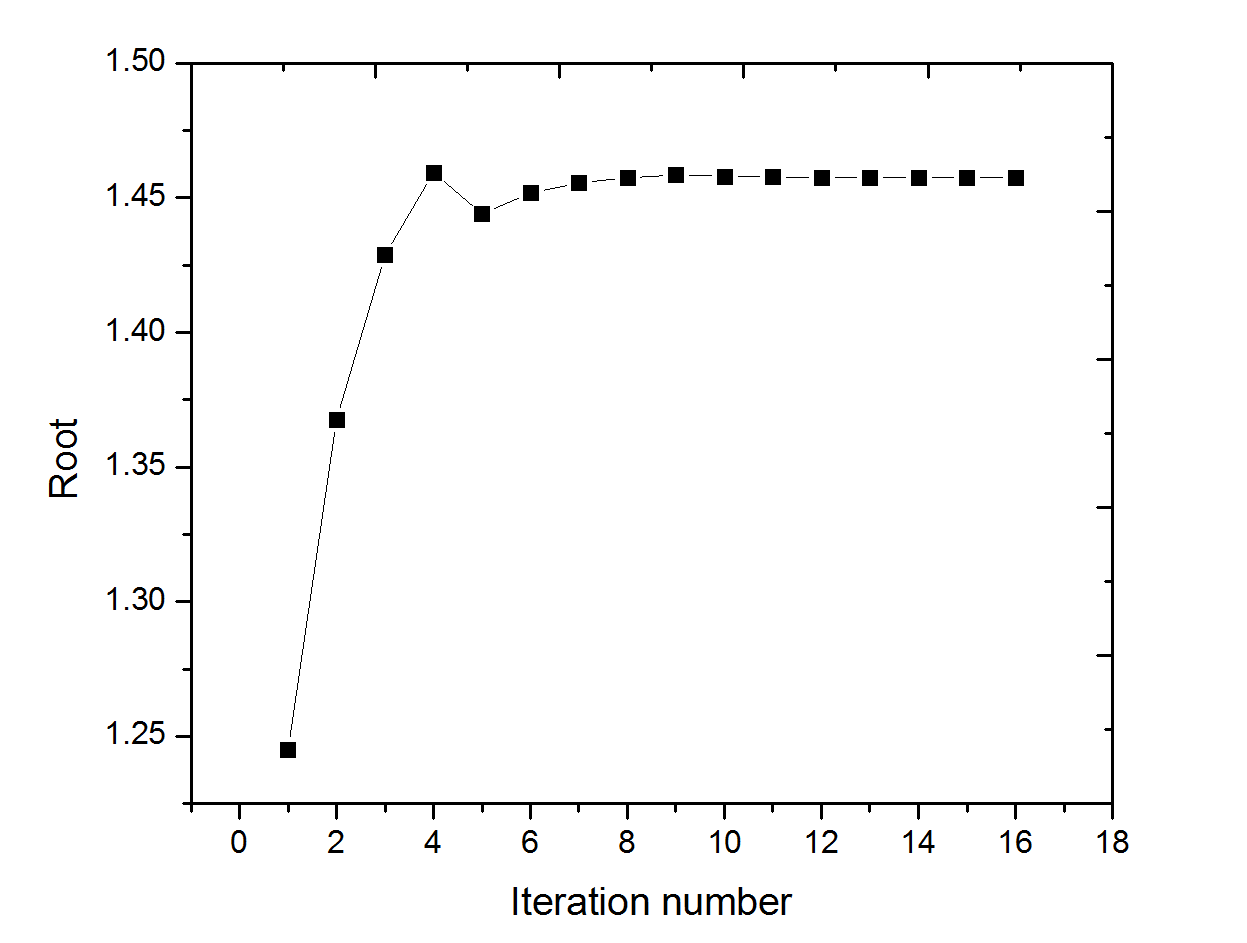
\includegraphics[width=0.5\textwidth]{root_6}
 \caption{Problem 6. Root vs interation number} 
 \end{figure} 
  \begin{figure}
 \centering 
 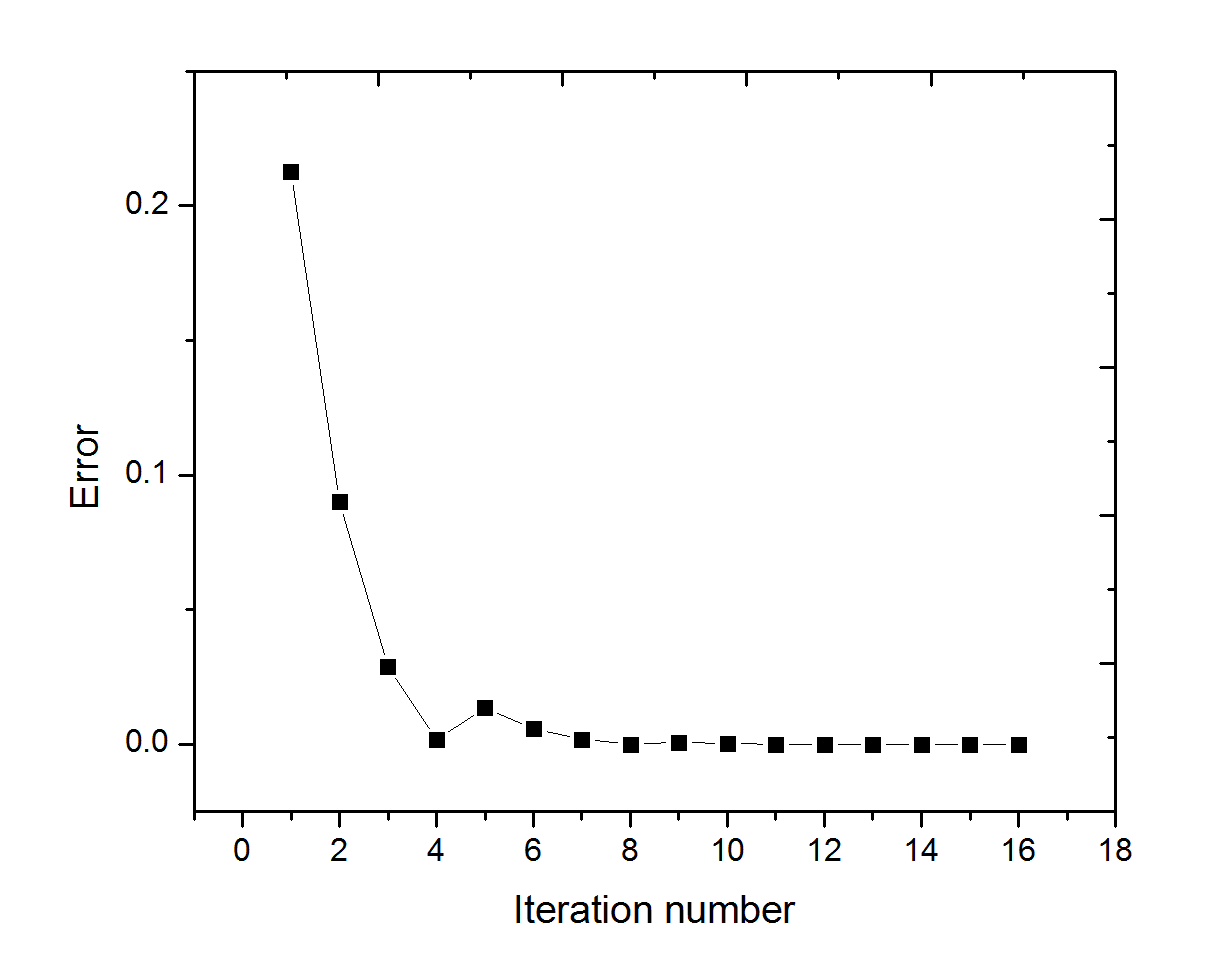
\includegraphics[width=0.5\textwidth]{error_6}
  \caption{Problem 6. Error vs interation number} 
 \end{figure} 

\hypertarget{problem_6_homework_checklist_2}{}
\subsection*{{Problem 7}}
\label{}
\begin{enumerate}
\item 
$f(x)=e^x+x^2-x-4 $  \\
$x=1.28868 $ \\
\item 
$f(x) =x^3-x^2-10x+7 $ \\
$x=0.68522 $\\
\item 
$f(x) = 1.05-1.04x+ln(x) $\\
$x= 1.10971$ \\

\end{enumerate}

\end{document}


